
\chapter{Descripción del Trabajo}
\label{cap:descripcionTrabajo}
En este capitulo se describe el framework de enemigos creado, mediante el diseño de componentes más sencillos. 
Primero se describirá el contexto y por tanto la utilidad de la herramienta, aquí se detallaran juegos analizados y sus características en común. Después se explicará que elementos la componen y por último se detallarán algunos ejemplos de uso. \\
\section{Contexto}
Como se señala en  \citet{Build_a_Bad_Guy_Workshop}, los enemigos bien diseñados son clave para evitar que los niveles queden planos y, en consecuencia, aburridos para el jugador.
\subsection{Enemigo}
Los enemigos son entidades programadas para enfrentarse al jugador y crear desafíos dentro del juego. Su diseño incluye características, comportamientos y habilidades diseñadas para interactuar con las mecánicas del juego y contribuir a la experiencia del jugador. \\
\subsection{Análisis de enemigos en videojuegos}
El análisis de diversos documentos muestra que la mejor forma de hacer que un enemigo destaque y de un gran potencial al juego es que tenga unos comportamientos únicos. Estos comportamientos han ido evolucionando con el tiempo volviéndose cada vez más sofisticados. Cada enemigo se define mediante una forma única de un conjunto de componentes bien seleccionados que permiten identificarlo y recordarlo.
Con dicha sofisticación, ha aumentado la complejidad del trabajo en el diseño. Para solucionarlo hemos propuesto una herramienta con la  composición indicada a continuación

\section{Composición}
En este trabajo, se ha decidido entender como enemigo a cualquier entidad que pueda repercutir de forma negativa en el jugador, esto significa que no se limita el concepto de enemigo a figuras típicas, como monstruos o soldados hostiles, sino que se amplía su definición a toda entidad que suponga un riesgo, dificultad o amenaza para el progreso o el bienestar del jugador dentro del juego, como pueden ser pinchos, lava o gotas de ácido.
Además separamos cada enemigo por comportamientos diferentes, implicando que elementos que clásicamente aparecen en conjunto, como la tubería y la gota de ácido o la bala y el pistolero, serán considerados como dos enemigos distintos.\\

\subsection{Máquina de estados finita}

La Máquina de Estados Finita (FSM, Finite State Machine) es el núcleo de la lógica que define el comportamiento de los enemigos en nuestro diseño. Cada enemigo tiene su propia FSM, configurada específicamente para representar sus patrones de acciones, reacciones y relaciones en el juego. La FSM organiza el comportamiento de los enemigos mediante estados y transiciones:
Los estados agrupan las acciones que el enemigo puede realizar en un momento dado.
Las transiciones permiten cambiar de un estado a otro y son activadas por sensores y emisores.\\
Estos conceptos (estados, sensores, emisores y eventos) se desarrollan con mayor detalle en los apartados siguientes.

El objeto enemigo se define mediante una máquina de estados finita y un script que contiene información relevante. A continuación, se describen ambos conceptos y sus propiedades.\\
\begin{figure}[h]
	\centering
	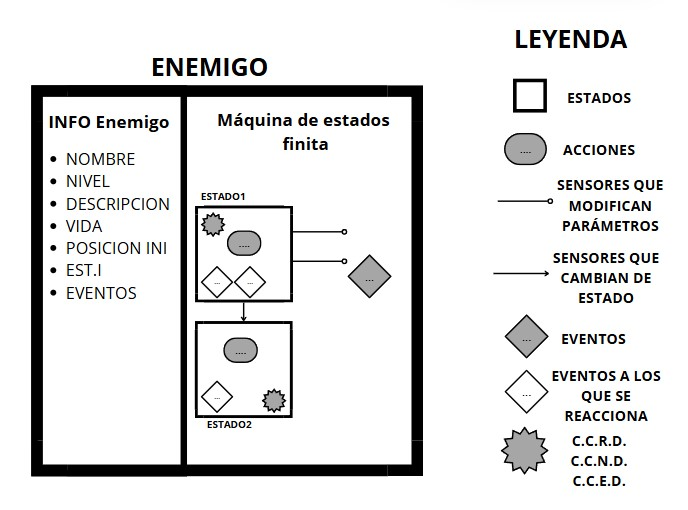
\includegraphics[width = 0.7\textwidth]{Imagenes/EnemigoGeneral.png}
	\caption{Enemigo General }
	\label{fig:EnemigoGeneral}
\end{figure}

\subsection{Estado}
Un estado dentro de la FSM se define como un conjunto de acciones y la posible activación de sensores y emisores, que en conjunto describen el comportamiento del enemigo. Las acciones pueden incluir uno o más tipos de movimiento compatibles entre sí, así como la capacidad de generar otros enemigos mediante un spawner.
Es importante destacar que la muerte del enemigo no se considera un estado dentro de la FSM. Este concepto se desarrolla en profundidad en el apartado de eventos.\\

Además cada estado contiene una lista que definen las dimensiones, tiempo de recarga y valor de daño de las cajas de colisión (explicadas en la sección de Daño).

\subsection{Acciones (Actuadores)}
Hace referencia a un conjunto de movimientos y habilidades que definen lo que un enemigo puede hacer en el videojuego. Esto incluye distintos tipos de desplazamientos y la capacidad de crear otros enemigos de forma independiente mediante spawners. Estas habilidades no siempre son compatibles entre sí, teniendo una tabla en la que se indicaran las relaciones entre ellas. Además no es necesario utilizar siempre todas las acciones de forma que a veces un enemigo podrá realizar un tipo de movimiento o usar un spawner de manera exclusiva, mientras que en otras podrá combinar varias habilidades según su diseño y complejidad. Esto permite adaptar las capacidades de los enemigos para diferentes situaciones en el juego.
\subsubsection{Spawner}
Capacidad que poseen los enemigos para generar otros enemigos independientes, es decir, poder crear nuevas unidades que actúan de forma autónoma dentro del juego.\\
Los spawners presentan características únicas dentro del sistema de enemigos, ya que su objetivo no es solo enfrentarse al jugador, sino también aumentar el número de amenazas de manera continua o en función de ciertas condiciones.
Implementar un spawner requiere establecer ciertas reglas de generación de enemigos, tales como la frecuencia de aparición, el número máximo de enemigos generados o si las unidades generadas son temporales o persistentes.
\subsubsection{Movimiento}
Podemos definir el término movimiento como el desplazamiento o cambio de posición de un enemigo dentro del juego. Sin embargo, el concepto de movimiento también puede aplicarse en el caso de enemigos que permanecen en una posición fija, haciendo referencia a la ausencia de éste. Los movimientos son fundamentales para definir el comportamiento de los personajes, ya que permiten la interacción con el jugador y el entorno.
A continuación se describen en una tabla todos los movimientos que se han considerado esenciales y en la figura \ref{fig:TablaCompatibilidad} podemos ver la compatibilidad entre ellos

\begin{table}[!h]
	\centering
	\begin{tabular}{|p{3cm}|p{4.5cm}|p{4cm}|p{3cm}|}
	\hline
	\textbf{Tipo movimiento} & \textbf{Descripción} & \textbf{Atributos} & \textbf{Ejemplo} \\ 
	\hline
	Movimiento Horizontal & Desplazamiento simple de lado a lado en el escenario. & Velocidad, aceleración & Woomba \\ 
	\hline
	Movimiento Vertical & Desplazamiento simple hacia arriba y abajo. & Velocidad, aceleración & Planta Carnívora \\ 
	\hline
	Quieto & El enemigo se mantiene en el sitio sin ninguna modificación aparente. & —  \\ 
	\hline
	Movimiento hacia un punto & El enemigo va hacia un punto. Puede ser a un punto fijo (estático) o a un punto en movimiento (dinámico). & Punto a seguir, actualizar, lista de puntos a seguir, velocidad, zona de puntos aleatorios. & N/A \\ 
	\hline
	Circular/Rotación & El enemigo describe trayectorias circulares a través de su movimiento. & Radio, velocidad angular, punto de rotación, sinusoidal, aceleración, rango de giro.  \\ 
	\hline
	\end{tabular}
	\caption{Tabla Movimientos}
	\label{tab:movimientos}
\end{table}

\begin{table}[h]
    \centering

    \renewcommand{\arraystretch}{1.5}
    \setlength{\tabcolsep}{4pt} % Reduce el espacio entre columnas
    \resizebox{\textwidth}{!}{
        \begin{tabular}{c|cccccc}
            & \cellcolor{gray!60} Movimiento Horizontal & \cellcolor{gray!60} Movimiento Vertical & \cellcolor{gray!60} Quieto & \cellcolor{gray!60} Movimiento hacia un punto & \cellcolor{gray!60} Circular/Rotación & \cellcolor{gray!60} Péndulo \\
            \hline
            \cellcolor{gray!40} Movimiento Horizontal &  &  &  &  &  &  \\ \addlinespace
            \cellcolor{gray!40} Movimiento Vertical & \cellcolor{green!70} &  &  &  &  &  \\ \addlinespace
            \cellcolor{gray!40} Quieto & \cellcolor{red!70} & \cellcolor{red!70} &  &  &  &  \\ \addlinespace
            \cellcolor{gray!40} Movimiento hacia un punto & \cellcolor{green!70} & \cellcolor{green!70} & \cellcolor{red!70} &  &  &  \\ \addlinespace
            \cellcolor{gray!40} Circular/Rotación & \cellcolor{green!70} & \cellcolor{green!70} & \cellcolor{red!70} & \cellcolor{green!70} &  &  \\ \addlinespace
            \cellcolor{gray!40} Péndulo & \cellcolor{green!70} & \cellcolor{green!70} & \cellcolor{red!70} & \cellcolor{green!70} & \cellcolor{green!70} &  \\ \addlinespace
        \end{tabular}
    }
    \caption{Matriz de compatibilidad de movimientos}
\end{table}


\subsection{Sensores y Emisores}
Podemos definir el término sensor como el elemento necesario para medir variables exteriores y enviar la información al enemigo. Los sensores permiten producir eventos. \\
Definimos Emisores como anónimo de sensor, es decir, es aquel elemento que envía información del enemigo al exterior.
Para explicar su funcionamiento se proponen algunos ejemplos.
\begin{table}
	\centering
	\begin{tabular}{|p{3cm}|p{4.5cm}|p{4cm}|p{3cm}|}
	\hline
	\textbf{Sensor/Emisor} & \textbf{Descripción} & \textbf{Atributos} & \textbf{Ejemplo} \\ 
	\hline
	Colisión  & Encargado de proceder al cambio de estado en caso de colisión. Puede especificarse la capa con la que se debe colisionar para proceder al cambio. &Capa con la que se colisiona. \\ 
	\hline
	Distancia & Encargado de medir la distancia entre un punto y otro, ya sea en uno de los ejes (X o Y) o la magnitud de la misma, y que en caso de que se llegue a una distancia deseada se procederá al cambio de estado.& Posición desde donde se detecta. Distancia Transición,Ignora paredes,Entidad Objetivo,Eje Objetivo: X o Y (en su defecto magnitud).  \\ 
	\hline
	Tiempo &Encargado de medir el tiempo transcurrido desde un inicio. Funciona a modo de contador &TiempoTransición \\ 
	\hline
	Daño &Encargado de detectar si algún volumen de colisión ha recibido algún impacto dañino &Volumen de colisión, recibe o no daño, aplica o no daño, daño persistente o no, . \\ 
	\hline
	Estado Jugador &El enemigo cambiará de estado dependiendo de las características del jugador & Struct Estado Jugador.
Ej: dirección a la que mira, si tiene seleccionada un arma counter del enemigo, si es vulnerable momentáneamente, si está siendo atacado por otros enemigo \\ 
	\hline
	Sonido &El enemigo mide el nivel de ruido que hace el jugador  y si supera cierto nivel lo detecta & Sensor de círculo por distancia. Hay que generar estímulos que se puedan recibir en algún momento\\ 
	\hline
	\end{tabular}
	\caption{Tabla Sensores/Emisores}
	\label{tab:Sensores/Emisores}
\end{table}
\subsection{Daño}
Cuando se habla de daño, el concepto de enemigo se deja a un lado y se habla de volúmenes de colisión.\\
Se define daño como la consecuencia negativa que recibe una entidad con respecto a su vida. Se produce como la consecuencia de que un volumen de colisión que emite daño colisione contra otro volumen de colisión que recibe daño.\\
Existen diferentes tipos de daño y parámetros específicos que determinan cómo los volúmenes de colisión reciben, emiten y procesan daño.
La primera consideración que hay que tener en cuenta es que el daño no es bidireccional, lo que implica que un volumen que recibe daño no tiene porqué emitir daño. Para reflejar esta diferenciación, en este trabajo se estructuran tres tipos de cajas de colisión:

\begin{itemize}
	 \item Caja de Colisión Recibir Daño (C.C.R.D): Áreas en las que el enemigo es vulnerable.
	 \item Caja de Colisión Emitir Daño (C.C.E.D): Áreas desde las que el enemigo inflige daño.
	 \item  Caja de Colisión No Daño (C.C.N.D): Zonas invulnerables del enemigo que no interactúan con el sistema de daño.
\end{itemize}
Además, estas cajas pueden activarse/ desactivarse y desplazarse dinámicamente en función del estado del enemigo o de las mecánicas del juego. Esto permite modelar comportamientos más complejos, como:
\begin{itemize}
	 \item Añadir funcionalidad a enemigos simples
	 \item Alterar zonas de ataque en función de animaciones o patrones.
	 \item  Optimizar las interacciones desactivando cajas no relevantes en momentos específicos del juego.
\end{itemize}
Además, se puede distinguir entre tres tipos de daños:
\begin{table}[!h]
	\centering
	\begin{tabular}{|p{3cm}|p{4.5cm}|p{4cm}|p{3cm}|}
	\hline
	\textbf{Nombre } & \textbf{Descripción} & \textbf{Atributos} & \textbf{Ejemplo} \\ 
	\hline
	Instantáneo & Se aplica de manera inmediata al jugador en el momento en que colisiona con C.C.E.D El daño se aplica de manera instantánea a la entidad la cual tenga el volumen de colisión que lo recibe

. &cantidadDaño
(si el valor es <0, instakill
). \\ 
	\hline
	Persistente & Este tipo de daño se mantiene mientras el volumen de colisión que lo recibe permanezca en contacto con el volumen de colisión que lo ocasiona.

 & ralentización movimiento, inmediata, daño residual \\ 
	\hline
	Residual & Representa el daño aplicado tras un impacto inicial, pero que permanece activo durante un corto período, infligiendo unas pequeñas cantidades de daño, incluso si el volumen de colisión ya no está en contacto con el volumen que inició el daño.

 & cantidadDaño
numerointervalos
tiempoIntervalos (cada cuanto hace daño)

&  Un enemigo con un ataque envenenante puede infligir daño progresivo durante unos segundos después de golpear al jugador.

 \\ 
	\hline
	
	\end{tabular}
	\caption{Tabla Daños}
	\label{tab:Daños}
\end{table}

\subsection{Eventos}

Un evento es una funcionalidad concreta y puntual que se activa mediante un sensor, está diseñado para ser procesado por cualquier entidad del juego que lo requiera.
Cuando se cumplen ciertas condiciones específicas, un evento puede desencadenar otro evento como consecuencia, creando una cadena de interacciones.
El uso de eventos contribuye a un diseño más orgánico y dinámico, ya que permite que los cambios de estado en los enemigos sean más evidentes para el jugador, mejorando así la experiencia de juego. Siendo especialmente visible en efectos gráficos y sonoros.\\

La muerte de un enemigo se implementa como un evento. Este evento se genera cuando el enemigo agota su salud o se encuentra en una condición específica de eliminación. Al activarse, se lanza para que otras entidades del juego lo procesen, representando el fin de la ejecución de la FSM y deteniendo cualquier acción del enemigo.

\subsubsection{Procesamiento de eventos}

Todos los eventos generados por sensores se manejan a través de una cola de eventos. Esta cola asegura que los eventos se procesen en orden de llegada (First In First Out, FIFO), evitando conflictos entre ellos. Cada enemigo evalúa los eventos de su cola de manera secuencial, ejecutando las acciones correspondientes antes de pasar al siguiente evento.

